% 2020-04-23 P.Shilane - update template for HotStorage'21
% 2020-09-22 J.Nider - updated template for Systor'21 (acmart.cls v1.73)
%
% This file is derived from "sample-sigconf.tex" of the acmart master template
% from 2018/07/16, v1.54
%
% This file should be compiled with
% "acmart.cls", "acmart.dtx", "acmart.ins", "ACM-Reference-Format.bst", v1.54
%
% See "2017 ACM Master Article Template":
% https://www.acm.org/publications/proceedings-template
%

% Do keep the \documentclass "anonymous" parameter until the review process finishes
%\documentclass[sigconf]{acmart}
\documentclass[sigconf,anonymous,10pt]{acmart}

\usepackage{enumitem}
\usepackage{url}
\usepackage{framed}

\usepackage{color}
\newcommand{\cred}[1]{\textcolor{red}[[#1]]}

% Copyright
% Pick the correct copyright notice that matches your rights form
%\setcopyright{none}
\setcopyright{acmcopyright}
%\setcopyright{acmlicensed}
%\setcopyright{rightsretained}
%\setcopyright{usgov}
%\setcopyright{usgovmixed}
%\setcopyright{cagov}
%\setcopyright{cagovmixed}

% DOI
\acmDOI{10.475/1234.5678}

% ISBN
\acmISBN{123-4567-24-567/08/06}

%Conference
\acmConference[HotStorage'21]{13th ACM Workshop on Hot Topics in Storage and File Systems}{July 27-28, 2021}{virtual conference}
\acmYear{2021}
\copyrightyear{2021}

%\acmArticle{4}
\acmPrice{15.00}

% These commands are optional
\acmBooktitle{Proceedings of the 13th ACM Workshop on Hot Topics in Storage and File Systems}
%\editor{John Doe}
%\editor{Jane Doe}

\begin{document}

\title{ObFS: A File System Translation Layer for Object Storage}

% Fill in your details. The \documentclass "anonymous" parameter keeps them hidden, remove it after the review process finishes
\author{Mania Abdi}
\affiliation{%
  \institution{Northeastern University}
  \city{Boston}
  \state{MA USA}
}
\email{abdi.ma@northeastern.edu}

\author{Peter Desnoyers}
\affiliation{%
  \institution{Northeastern University}
  \city{Boston}
  \state{MA US}
}
\email{p.desnoyers@northeastern.edu}

% The default list of authors is too long for headers.
%\renewcommand{\shortauthors}{M. Abdi and P. Desnoyers}

\begin{abstract}
We present ObFS, a novel log-structured file system designed to use S3-like write-once object storage as its underlying media.
It is based on traditional translation layer---rather than file system---mechanisms, using in-memory metadata, logical journaling in out-of-band headers, and periodic metadata checkpoints.
ObFS is a single-client file system over remote storage, targeted to containerized applications which typically use block storage for persistent volumes.
Its novel structure allows straightforward implementation of snapshots, cloning, and overlays, all highly useful for this use case.
A preliminary FUSE-based implementation is described.
\end{abstract}

%% Note: Classification and Keywords are only required for the camera-ready version

%
% The code below should be generated by the tool at
% http://dl.acm.org/ccs.cfm
% Please copy and paste the code instead of the example below.
%
\iffalse
\begin{CCSXML}
\begin{CCSXML}
<ccs2012>
   <concept>
       <concept_id>10011007.10010940.10010941.10010949.10003512</concept_id>
       <concept_desc>Software and its engineering~File systems management</concept_desc>
       <concept_significance>500</concept_significance>
       </concept>
   <concept>
       <concept_id>10010520.10010575.10010581</concept_id>
       <concept_desc>Computer systems organization~Secondary storage organization</concept_desc>
       <concept_significance>300</concept_significance>
       </concept>
 </ccs2012>
\end{CCSXML}
\ccsdesc[500]{Software and its engineering~File systems management}
\ccsdesc[300]{Computer systems organization~Secondary storage organization}
\keywords{Object storage, Network file system}
\fi

\maketitle

\sloppy

\section{Introduction}

ObFS is a local file system designed to store data and metadata on S3-like write-once object storage.
It achieves the speed of a local file system by using objects as containers for file system data structures; this is in contrast to 1:1 object:file mappings such as S3FS~\cite{kovacs_amazon_2020}, which suffer from limited S3 semantics and in particular the need to rewrite entire objects for any modification.

It targets persistent volumes for containerized applications, which at present typically make use of local file systems over remote block storage\footnote{E.g. a significant majority of current Kubernetes remote persistent volume providers implement block rather than file storage: \url{https://kubernetes.io/docs/concepts/storage/volumes}}. 
Remote access is highly desirable in this use case, both for reliability (e.g. replication) and flexibility in scheduling; however although multi-client access may be useful, the widespread use of block storage indicates that it is by no means a requirement.
Although ObFS is a single-client file system, the externally-visible objects written by ObFS form a consistent snapshot, providing visibility from external systems in a way not possible with typical local file systems over remote block storage.

ObFS takes a novel approach, leveraging mechanisms traditionally used in flash translation layers to take best advantage of the write once / read many / delete semantics of S3 object storage.
It logs data and metadata to a stream of objects, with each object containing data from write operations as well as a header analogous to the out-of-band (OOB) data region in a flash page.
These headers hold a write-optimized logical journal of metadata modifications, however the primary metadata representation is in-memory, with periodic checkpoints\footnote{%
  As the file system grows, in-memory metadata may be evicted and demand-loaded from prior checkpoints; see later sections for details.} to the object stream.

The lightweight nature of logical journaling (roughly 40 bytes per operation in our current implementation) avoids the metadata write expansion found in most log-structured file systems, where a single block write may trigger a cascade of block writes to update indirect blocks, inodes, and directories all the way up the tree~\cite{hitz_file_1994}.
Metadata updates are instead batched and written at fairly long intervals, with a tradeoff between the overhead of these updates and the time taken by log roll-forward during crash recovery.

As a log-structured system, ObFS easily supports not only snapshots but creation of clone file systems off a single base.
In addition we describe a directory structure which supports a form of ``native overlay'' or multiple inheritance, allowing a file system to be constructed of the union of an ordered list of precursors.

ObFS differs significantly from most previous file systems:
\begin{itemize}[nosep]
\item It combines journaling with log structure, a combination only found in F2FS~\cite{lee_f2fs_2015}, and there to a limited extent.
\item It is a ``containerless'' file system. In contrast to most file systems which use the same container structure to hold the contents of both files and directories, ObFS (like e.g. BeTRFS~\cite{jannen_betrfs_2015} maintains metadata structures separate from the files themselves, and writes them in a simple serialized format.
\item It is non-block-based, taking advantage of 64-bit systems to use byte rather than block pointers\footnote{This is a consequence of several design decisions; whether it is of practical value remains to be seen}.
\end{itemize}

ObFS is at a proof-of-concept stage at present: we have implemented a FUSE prototype over S3.
Full file system functionality has been implemented (including garbage collection and checkpointing, which are necessary for normal use) but advanced features are still under development.
%In the remainder of this paper we describe ObFS, evaluate our prototype, and survey related work.

\section{The ObFS File System}

ObFS is based on the following principles:

1. Metadata is designed to be used in memory, not from storage.
Files are maps from extents within the file to extents within objects, and directories are maps from names to inode numbers and ancillary information.
Metadata objects are serialized into checkpoints and may then be flushed from memory and demand-loaded later, but the metadata serialization format is not designed to be mutable.

2. Data and metadata is persisted in a stream of objects tagged with sequence numbers as numeric prefixes, allowing efficient internal representation of object names.
Each object encodes a consecutive sequence of file system operations, allowing a consistent prefix to be recovered after failure even if multiple object writes are in progress at the time of failure.

3. Files, directories, and other file system objects (symlinks, special files) are identified by inode number.
These numbers are opaque identifiers and do not identify location, but instead are assigned from an incrementing counter.

4. Each object contains a logical journal of individual file system operations, described below, plus a data region containing the data for write operations in the journal.

\begin{figure}
\begin{framed}
{\footnotesize 
\begin{verbatim}
object "vdisk.0000":
  INODE num=1 mode=S_DIR|0777, size=0, uid/gid, timestamp
  CREATE parent=1 inum=2 name="file.txt"
  INODE num=2  mode=S_REG|0777, uid/gid, size=0, timestamp
  DATA 11 offset=0 dataptr=0 len=15 newsize=15
  --
  this is a test\n
\end{verbatim} }
\end{framed}

  \caption{ A trivial ObFS file system. \rm The root directory is inode 1; it contains a single file, ``file.txt'', with a 15-byte write starting at offset 0 in the object data segment.} 
  %(S\_REG is the POSIX mode flag for a ``regular'' file)}
  \label{figure:journal1}
\end{figure}

\begin{figure}
\begin{framed}
 {\footnotesize
\begin{verbatim}
object "vdisk.0001":
  CREATE parent=1 inum=3 name="dir1"
  INODE num=3 mode=S_DIR|0777, uid/gid, size=0, timestamp
  DATA num=2 offset=15 dataptr=0 len=15 newsize=40
  --
  this is another test\n
\end{verbatim} }
\end{framed}
  \caption{Second data object. \rm Creates subdirectory \texttt{/dir1} and adds 15 bytes to \texttt{/file.txt}.}
  \label{figure:journal2}
\end{figure}


\begin{figure}
\centering
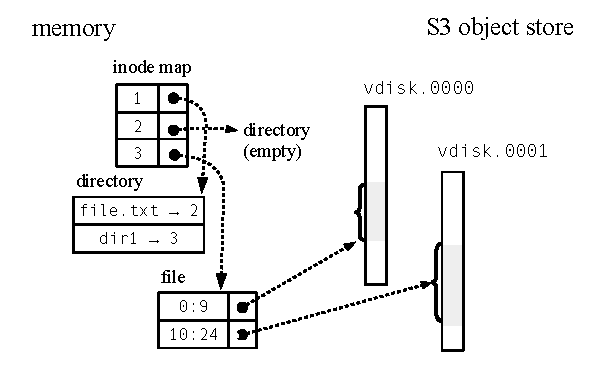
\includegraphics[width=0.95\columnwidth]{figures/obfs.pdf}
\caption{Relationship of in-memory structures and S3 objects for file system shown in Figures \ref{figure:journal1} and \ref{figure:journal2}.}
\label{figure:picture}
\end{figure}

\subsection{Logical Journal Format}

A trivial example of an ObFS file system may be seen in Figure~\ref{figure:journal1}.
It contains a journal of the following operations:
\begin{itemize}[nosep]
\item Modify root directory properties (inode 1) to set permissions, UID/GID, and timestamp
\item Create an entry for a new file, \texttt{/file.txt} in the root directory
\item Set inode properties for the file
\item Write 15 bytes to the file
\end{itemize}

At mount time the log will be replayed; when complete the root directory will have a single entry [\texttt{"file.txt"} $\rightarrow$ 2], and the file identified as inode 2 will have a single extent in its map, with offsets $[0\ldots 14]$ mapped to offset 0 in the data section of object 0.
In Figure~\ref{figure:journal2} we see the second object in the stream, journaling the creation of an empty directory (\texttt{/dir1}) and the write of 15 more bytes to \texttt{/file.txt}; again these will be reflected in in-memory data structures after journal recovery during the mount process.

\begin{table}
  \begin{tabular}{l|l}
    Operation & \rule{4em}{0pt} arguments \\
    \hline
    INODE & inum, mode, uid/gid, rdev, mtime \\
    CREATE & parent inum, inum, name \\
    RENAME & inum, parent inum1, inum2, name1, name2 \\
    TRUNC & inum, new size\\
    DELETE & parent inum, inum, name \\
    SYMLINK & inum, target\\
    DATA & inum, file offset/len, obj offset, new file size\\
    \hline
  \end{tabular} \vspace{0.5\baselineskip}
  \caption{ObFS journal entry types}
  \label{table:journal}
\end{table}

The full list of seven journal entry types may be seen in Table~\ref{table:journal}.
We believe that they are sufficient for basic POSIX file system functionality, although our implementation has taken some liberties with timestamps (we assume \texttt{noatime} mounts) and we have not yet implemented reference counting for hard links in either the in-memory or serialized metadata formats.

Figures~\ref{figure:journal1} and \ref{figure:journal2} show back-end storage objects which are ridiculously small, for illustrative purposes.
In practice objects would be written when either (a) a default size has been reached (e.g. 8-16\,MiB), (b) an idle timeout has passed (e.g. 1s), or (c) a synchronizing operation (\texttt{fsync}, etc.) is performed.
The file system may be operated in an unsafe mode by either ignoring synchronizing operations entirely, in which case failure may cause data and operation loss but will not result in an inconsistent file system, or by logging to local high-speed storage, in which case synchronized data may be lost in the case of catastrophic failures.

\subsection{In-memory metadata}
Although in-memory data structures for a file system may be considered implementation details rather than architecture, their functionality is central to the architecture of ObFS.
Our description of these structures is provided in order to explain this functionality in a straightforward fashion, rather than to constrain implementation\footnote{For instance, in a proper in-kernel VFS implementation the structures described would no doubt be ``absorbed'' into existing kernel data structures.}.

ObFS supports the standard UNIX/POSIX file system objects: files, directories, symbolic links, and various classes of special files (e.g. character devices) with no file system functionality.
All objects (in the OO sense) have basic metadata such as uid/gid and timestamps; with the addition of a device number this is sufficient for the special file types.
This object is extended with the following information for the remaining types:
\begin{itemize}[nosep]
\item \textbf{Symbolic link:} a single string, the link target.
\item \textbf{Directory:} a map from strings (i.e. names) to integer inode numbers.
\item \textbf{File:} a byte-granularity interval map from offset ranges within the file to (object, offset) pairs indicating the location of the data in an S3 object\footnote{We explicitly call these ``S3 objects'' here to differentiate from in-memory objects, however other S3-like services providing named objects may of course be used.} from storage objects; however , with S3 objects identified by their integer sequence number.
\end{itemize}

Finally an inode table is used to map inode numbers to objects; path traversal thus iterates between accesses to this table and to individual directories.

\subsection{Checkpoints}

If ObFS were to do nothing but log operations to storage then mounting a file system would soon become unwieldy, requiring the playback of all operations performed on the file system to date.
To avoid this we periodically checkpoint metadata to storage so that the file system may be mounted by locating the most recent checkpoint, loading that into memory, and then rolling the journal forward from that point.
Note that a clean unmount will perform a checkpoint after all writes are complete, eliminating any recover overhead at mount time.

As the file system grows, the memory requirements for in-memory metadata may grow excessive.
This may be addressed by demand-loading metadata from the most recent checkpoint, and evicting unmodified metadata objects from memory when necessary.
This requires a mechanism to map an inode number to its location in the checkpoint: the two obvious possibilities are (a) a mapping table in the checkpoint, or (b) appending the information to directory entries.
Our current design stores an inode number to location map in the checkpoint, in part because this mapping is needed during garbage collection, when the identity of the parent directory may not be known.
We expect to revisit this decision as we gain experience with larger file systems, as performance may suffer if this table grows too large to be held in memory.

With further growth of a file system the overhead of writing checkpoints will increase.
If a fixed checkpoint interval is maintained, then metadata write overhead will go up as the ratio of modified to total metadata shrinks.
However, if the checkpoint interval is allowed to expand proportionally to reduce this overhead, mount time will suffer.

This may be addressed by keeping multiple partial snapshots.
Rather than implementing a complex garbage collection mechanism we use a simple FIFO method, keeping the last N checkpoints and copying any un-replicated data from the oldest checkpoint when we make a new one.
The need to keep separate inode maps for each snapshot limits the number of snapshots which may be maintained in practice, and alternate methods may be needed to support volumes of more than a few tens of millions of files.

\subsection{Garbage Collection}

ObFS has been tested with a simple Greedy cleaning algorithm, selecting the least-utilized objects, reading and re-writing any remaining live data before object deletion.
This is known to be optimal for uniform memoryless workloads~\cite{yang_optimality_2015}, but to perform poorly when workloads are skewed or correlated~\cite{desnoyers_analytic_2014}. 
We therefore include several well-known techniques which greatly improve its performance on realistic workloads:

\textbf{Dual write frontiers:}~\cite{lin_dual_2012} In realistic workloads, data which has survived long enough to be copied during garbage collection has a longer expected time-to-live than new writes.
  ObFS garbage collection output is written into separate objects, implicitly performing hot/cold data segregation.

\textbf{Write coalescing:} The hottest data items will be overwritten before an object is written to storage.
  By merging data and metadata in an object before it is written out, this space may be reclaimed without any copying, or even writing it in the first place\footnote{This is not yet implemented in our prototype.}.

\textbf{Hysteresis-based batching:} Optimal cleaning of skewed workloads requires allowing blocks containing hot data to ``age'' to lower utilizations than those containing cold data~\cite{desnoyers_analytic_2014}.
  To do this optimally requires extensive bookkeeping; however in practice the simple hysteresis mechanism we use achieves most of its benefits, deferring cleaning until a low-water mark is reached, then cleaning until a high-water mark is reached.

To identify live data we read the DATA records from the object header, and for each check that the current extent map still refers to the same location.
If the relevant inode is in memory it may be looked up directly; if not, the inode location map is used to demand-load it.
Although not implemented in our current prototype, we plan to segregate metadata loaded for garbage collection and free it at the end of the cycle.

Finally we note that ObFS objects contain metadata such as directory and inode information (e.g. CREATE and INODE records) as well as data.
Garbage collection must therefore either (a) only consider objects for deletion which are older than the most recent full checkpoint, or (b) create a new checkpoint before deletion.
Our current prototype chooses option (b), checkpointing metadata before beginning a garbage collection cycle.

\subsection{Additional features}
We are extending ObFS to support snapshots, clones of a base file system image, and "native overlay"---a form of clone based on multiple parent file systems.
We describe these briefly due to space limitations.

\noindent \textbf{Cloning:} The object stream for a cloned volume looks almost exactly like that for a simple ObFS file system, with objects older than a certain sequence number belonging to the base image, and later objects belonging to the clone, using a different prefix for object names.

\noindent \textbf{Snapshots:} A snapshot is just a specific object in the stream and its predecessors.
Garbage collection continues in the presence of snapshots; however objects containing data referenced by snapshots are not deleted until those snapshots have been removed.

\noindent \textbf{Overlay:} This is performed via an ordered merge of the metadata from several underlying file systems\footnote{This involves translating inode numbers and object sequence numbers; lack of space prohibits a full explanation.}, which may then be written as the initial checkpoint of the merged volume.
Although this is a heavier-weight process than union mount, the resulting file system will operate at native speed.

%\cite{10.1109/SMARTCOMP.2014.7043841}


\section{Implementation and Evaluation}

Our ObFS prototype is a FUSE file system implemented in roughly 2000 lines of C++.
It performs garbage collection and checkpointing, but does not yet implement snapshots, clone, overlays, or partial checkpoints.
We have verified its functionality against a local S3 object store\footnote{Based on Ceph Rados Gateway (RGW).}, but do not yet have performance results.

\section{Related Work}
The closest related work to ObFS is likely ObjectiveFS\footnote{\url{https://objectivefs.com}}, a multi-client file system over S3 which appears to provide NFS-like close-to-open consistency.
Like ObjectiveFS, it uses S3 as a data and metadata store rather than providing 1:1 mapping, achieving performance comparable to or better than NFS, however its structure and algorithms have not been publicly disclosed and are not known to the authors.

Log-structured file systems have a long history, from LFS~\cite{rosenblum_design_1991} and WAFL~\cite{hitz_file_1994} through more recent systems such as F2FS~\cite{lee_f2fs_2015}.
To the authors' knowledge F2FS is the only log-structured file system to date to use write-optimized journaling and recovery-time roll-forward to reduce the cost of metadata updates.
However the use of journaling in F2FS is very limited, as opposed to its pervasive use in ObFS.

The lack of a standard on-media container structure in ObFS is unusual but not unprecedented, and can be compared with BetrFS~\cite{jannen_betrfs_2015} and its use of a schema for data and metadata over an underlying key-value store.
In both cases the lack of directory containers is a result of fundamental architectural decisions, and does not in itself confer any benefits.

Finally, ObFS owes a debt to several decades of research on Flash Translation Layers.
In particular, at the time of development of the first log-structured file systems with garbage collection (e.g. LFS~\cite{rosenblum_design_1991}, Envy~\cite{wu_envy_1994}) there was no prior art for understanding the behavior and costs of garbage collection.
In the time since then great strides have been made in understanding this process, both its risks (i.e. catastrophic performance loss under sustained random write workloads), how to ameliorate them in theory, by segregating data by expected lifetime~\cite{lee_last_2008}, and practical methods for doing so, such as multiple write frontiers~\cite{lee_f2fs_2015} and cleaning hysteresis.

\section{Future Work}
Our work on ObFS is at an early stage, and we are just beginning to evaluate its performance.
In addition to this, further work is needed to explore aspects of ObFS design and possible improvements:

\textbf{Defragmentation:} Files in ObFS have the potential to become  fragmented, especially when byte-aligned writes are used\footnote{E.g. in a FUSE implementation, as opposed to the block-aligned writes which would be seen with an in-kernel VFS-level implementation.}; in addition frequent synchronization may result in the creation of numerous small objects.
Additional study is needed to determine the extent to which fragmentation occurs and its performance impact, to what degree it is controlled by write merging and batched garbage collection, and whether further measures are needed.

\textbf{Local storage:} ObFS can make use of high-speed local storage in two ways: either buffering synchronization operations for \texttt{fsync}-heavy workloads, or as a full local cache; we plan to explore both.

\textbf{Local block devices:} ObFS may be adapted for use over local block devices with no need for garbage collection, using a bitmap allocator and objects spread across discontiguous extents.
We refer the reader to Blizzard~\cite{mickens_blizzard_2014} for a description of how ``hole-plugging'' allocation may be used in such a system, by checkpointing the allocation bitmap, allowing the recovery process to replicate post-checkpoint allocation decisions.

\textbf{Persistent memory:} The block-less structure of ObFS suggests that it may be suited for use with persistent memory.
Our longer-term plans for ObFS include examination of whether there are any performance or functionality advantages to non-block file systems either in the kernel or in library operating systems.

\textbf{Container-to-host file systems:} One method of hardening containers is to narrow the interface to the operating system.
Container security remains a significant concern~\cite{sultan_container_2019}, with one possible solution being that of narrowing the system call interface, by e.g. implementing the file system within the container.
ObFS would allow the host to provide a narrower write-once object interface, while giving snapshot-level host visibility not possible with most block file systems.

\section{Conclusion}
ObFS represents a novel direction in file system organization.
It is at an early stage at present, but is already showing promise.

\iffalse
\section*{Acknowledgments}
Acknowledgments are for the camera-ready version only. Please do not include them in your submission.
Need to mention Red Hat and NSF small grant.
\fi

\bibliographystyle{ACM-Reference-Format}
\bibliography{objectfs}
\end{document}

\iffalse
ObjectFS is based on the following principles:
1 - logical journaling combined with a log-structured file system
2 - separation of metadata from file system contents
3 - overlaying or "patching" of directories and files


We explain ObjectFS in stages, starting with the simplest example with a single file stored in a single object, as seen in Figure~\ref{fig1}.
The object is split into two sections: the header, containing a logical journal, and the data section, containing bytes written to files.
Each object has a 64-bit sequence number, which is used as the suffix of the object name.


As files are overwritten or deleted, the data stored in older objects will become outdated and a garbage collection process will be needed.
We can keep track of the utilization of each object in memory, decrementing it whenever an extent in that object is overwritten or the file is deleted.
The garbage collection logic then identifies objects to clean, and retrieves and rewrites any remaining live data from these objects before deleting them.


<<<< put this later
we retrieve the object header and get the list of inode extents originally stored in that object; we can then look up the current mapping for that range of the file to determine if the data is still live and needs to be copied before object deletion.
<<<<



Up to this point we have assumed that all file system metadata --- inodes, directories, and file extent maps --- is held in memory and accessed there when necessary.
For larger file systems we will want to be able to limit the amount of data which must be held in memory, leading to the structure shown in Figure X.
In each directory entry we indicate not only the inode to which it maps, but the byte offset and length of where the full object (including dirents or file extent list) may be found in the checkpoint.
When traversing a path, if we reach an object which is not resident in memory, this information will allow it to be demand-loaded, and the operation may then continue as if all information had been memory-resident.


File system specifics

ObjectFS supports 4 object types: files, directories, symbolic links, and ``other'', a catchall for devices, pipes, and sockets.
At present it uses the seven journal entry types shown in Table X.
These entries are extremely compact, using less than 40 bytes each assuming a mean name length of 16 bytes.
As a result, metadata-heavy workloads such as small file creation and deletion result in very little I/O---almost all the work is performed in memory, at the time of the operation and possibly a second time if the log is replayed.


-----


File system layouts can be categorized in a number of different ways, one of the most significant of which is where they write modified data:
update-in-place file systems translate multiple overwrites of a file offset into multiple rewrites of the same underlying storage, while copy-on-write [out out-of-place update] file systems allocate new storage locations for every modification.

"Pure" update-in-place file systems such as FFS or ext2 are vulnerable to file system corruption if failures occur during the write process, so modern file systems of this type incorporate \emph{journaling}---a write-ahead log allowing changes to be made atomically.

[say more about out-of-place write]

File system data structures can be classified as \emph{read-optimized} or \emph{write-optimized}, or occasionally both.
By \emph{read-optimized} we mean structures like the inodes, indirect blocks, and directories of a traditional Unix file system, where any destination may be reached via a combination of indirection and limited searching, i.e. within a directory.
In contrast, in purely \emph{write-optimized} structures such as a journal there are no pointers or indexes; instead exhaustive search must be used to locate any specific piece of information, for instance the most recent copy of a specific inode.
Rather than repeatedly searching the journal for different items, we instead examine it once at recovery time and recover an up-to-date view of all information in the journal.
[ext4-lazy]

Interestingly, few copy-on-write file systems use any form of journaling.
Instead out-of-place writes are used to create a new read-optimized structure, and then the file system state is atomically shifted to this new structure.
In [LFS they do .., in WAFL, in ZFS, in Btrfs]


\fi
